\section{作业题目：结构力学基础与技巧班第3次作业（材料力学回顾）}
\begin{analysisbox}
弯矩图、剪力图和轴力图要先确定支座反力，再按截面法分段。符号约定要前后一致，最大应力或变形应结合截面几何量与材料参数检查量纲。
\end{analysisbox}
\subsection*{第 1 页转写}
第了次作业一一材料力学回顾

材料力学回顾作业及答案

、画剪力图和弯矩图

30kN

15kN/m

1m

3m

(a)

(b)

4kN-m

40kN

30kN-m

0.2kN/m

1m

10m

4m

(c)

(d)

20kN-m20kN

6kN.m

5a

3m

(e)

(f)
\begin{figure}[H]\centering
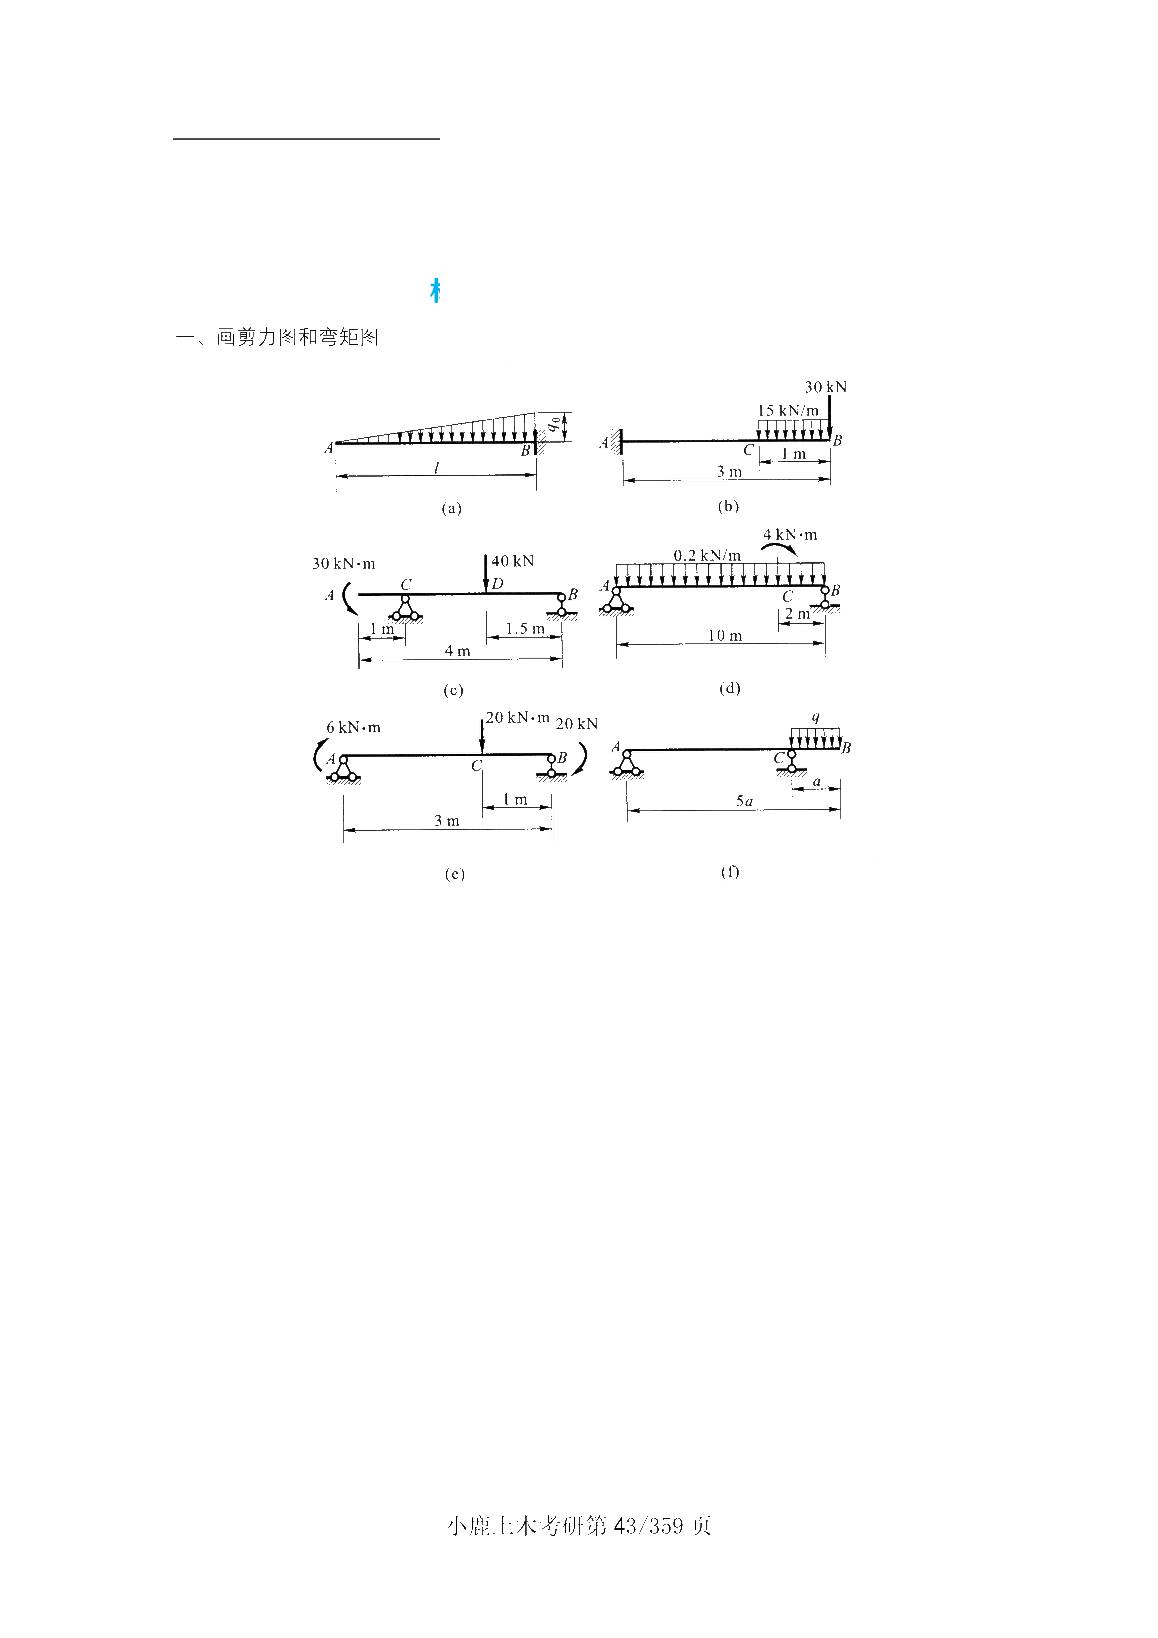
\includegraphics[width=0.92\textwidth]{figures/src06_p001.jpg}
\caption{结构力学基础与技巧班第3次作业（材料力学回顾） 第 1 页清理图形页}
\end{figure}
\subsection*{第 2 页转写}
试利用荷载集度、剪力和弯矩间的微分关系作下列各梁的剪力图和弯矩图。

15kN,10kN.m

5kN/m

1m

2.5m

1m

2m

(a)

(b)

M.

2M.

3a

5a

3a

(c)

(d)

IF

4kN m

20kN m

4kN/m

DA

4m

(e)

(f)

2kN/m

250kN\_250kN

10kN/1

6m

(g)

(h)

试作下列具有中间铰的梁的剪力图和弯矩图。

M.

Db=

(a)

(b)
\begin{figure}[H]\centering
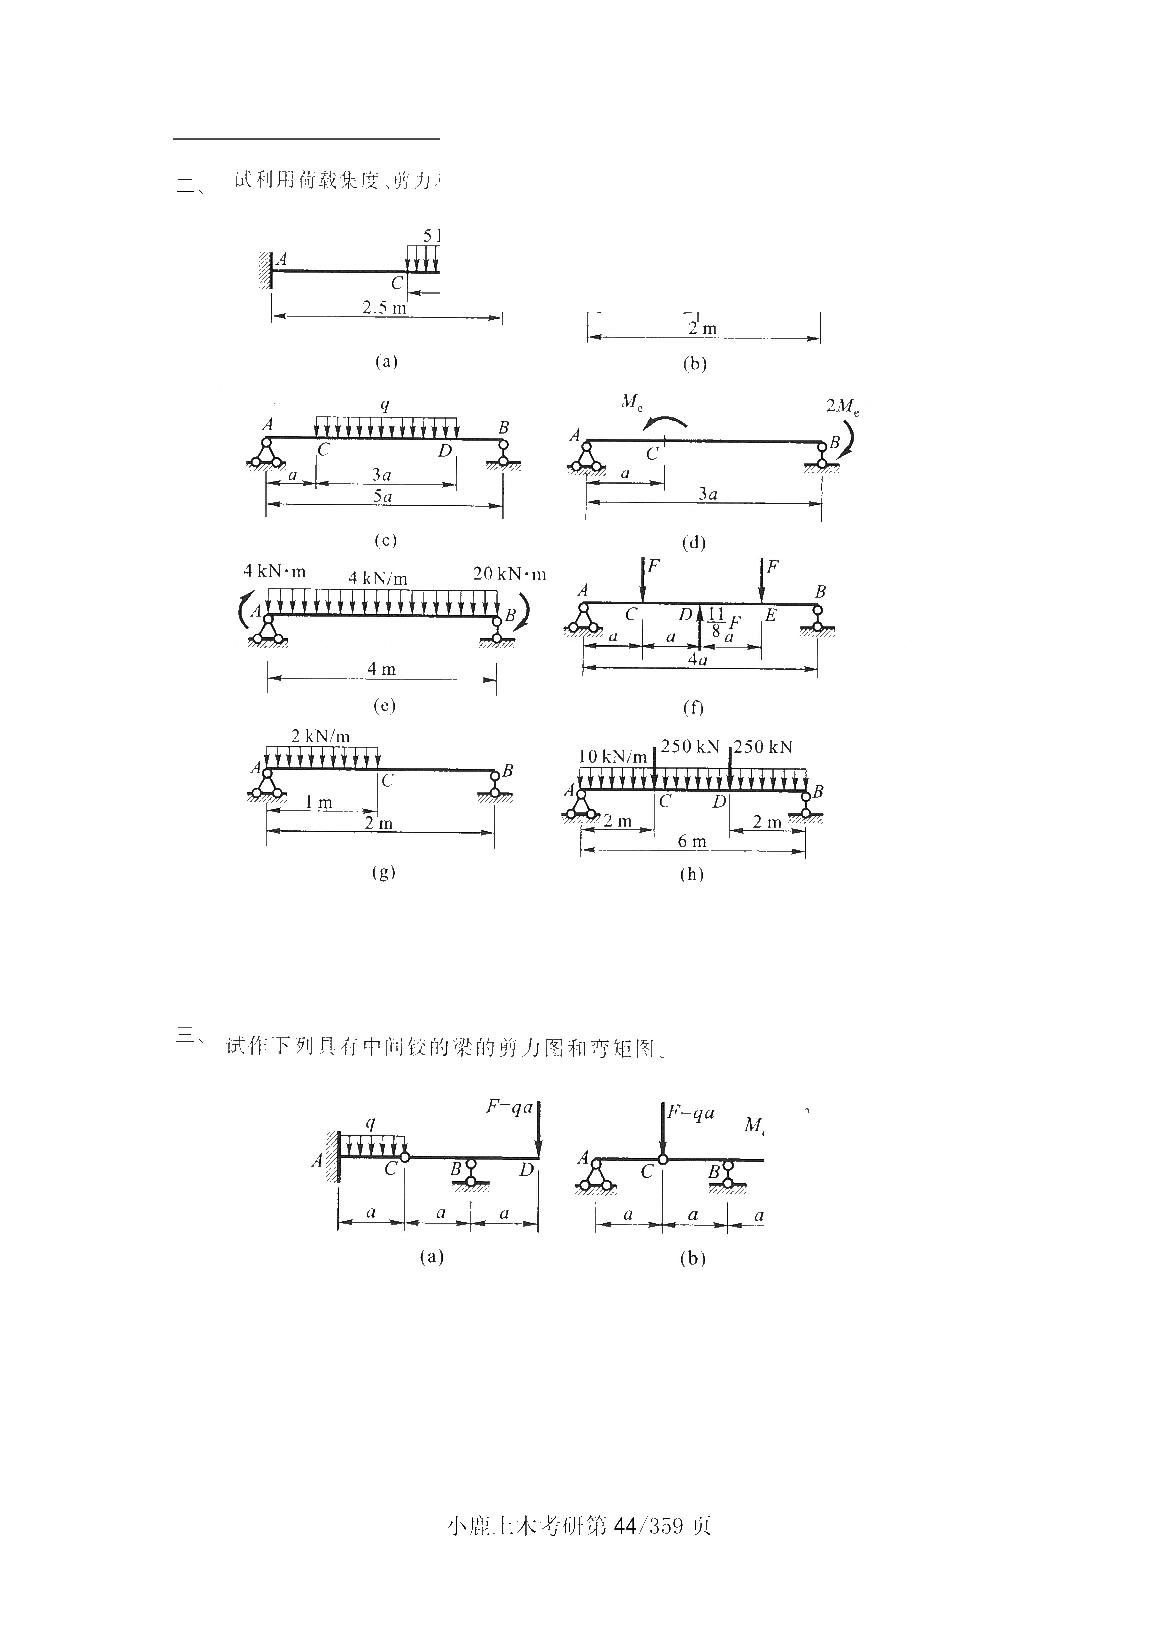
\includegraphics[width=0.92\textwidth]{figures/src06_p002.jpg}
\caption{结构力学基础与技巧班第3次作业（材料力学回顾） 第 2 页清理图形页}
\end{figure}
\subsection*{第 3 页转写}
(0)

的如ca-1)

(1-W)

M=0, M= -\% .X

考矩势内因如国a$\alpha$-1) (a-3) 手,

(o-3)

(A-2)

70

=0, M+J0$\times$(7-X)+15X1$\times$(-)$\ge$0

130

50=15

M=-1575+75-
\begin{figure}[H]\centering
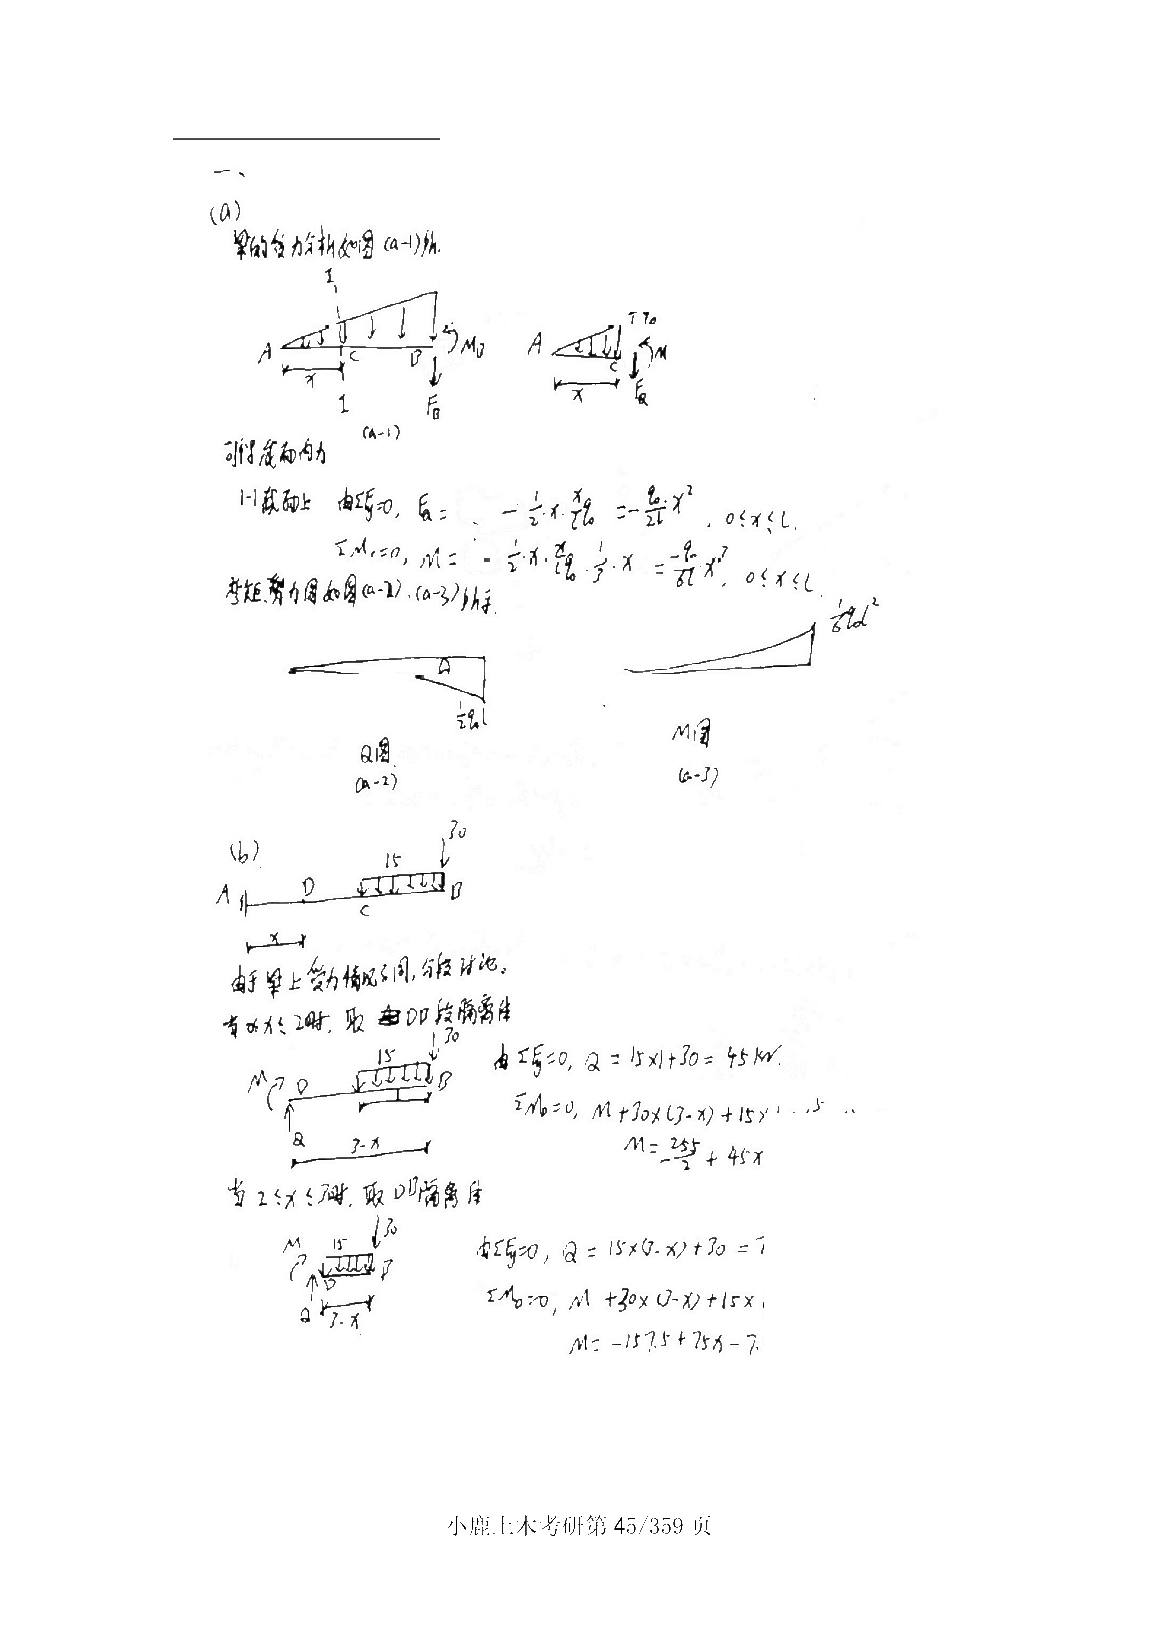
\includegraphics[width=0.92\textwidth]{figures/src06_p003.jpg}
\caption{结构力学基础与技巧班第3次作业（材料力学回顾） 第 3 页清理图形页}
\end{figure}
\subsection*{第 4 页转写}
(4sT-1275)1mm，05x52.

(675-15x)1m, 22 x53

1(-7.5+-525

1275

375

Qi. (w)

由平衡轻IMg20,F.了= Jo+to xls，Fa=Jo.

500, 后垢 =o, Fg= 10 r.

取AC较随离件，于AC泛旁力为0,可好Me=30l-m.

连接 B. C点考近, 中Mp=0 , 充nc较学范明上发加针力 \%kv 作个用无响文弹上的报因,

中 本+tox 了-Jokw.m.

30

30

10
\begin{figure}[H]\centering
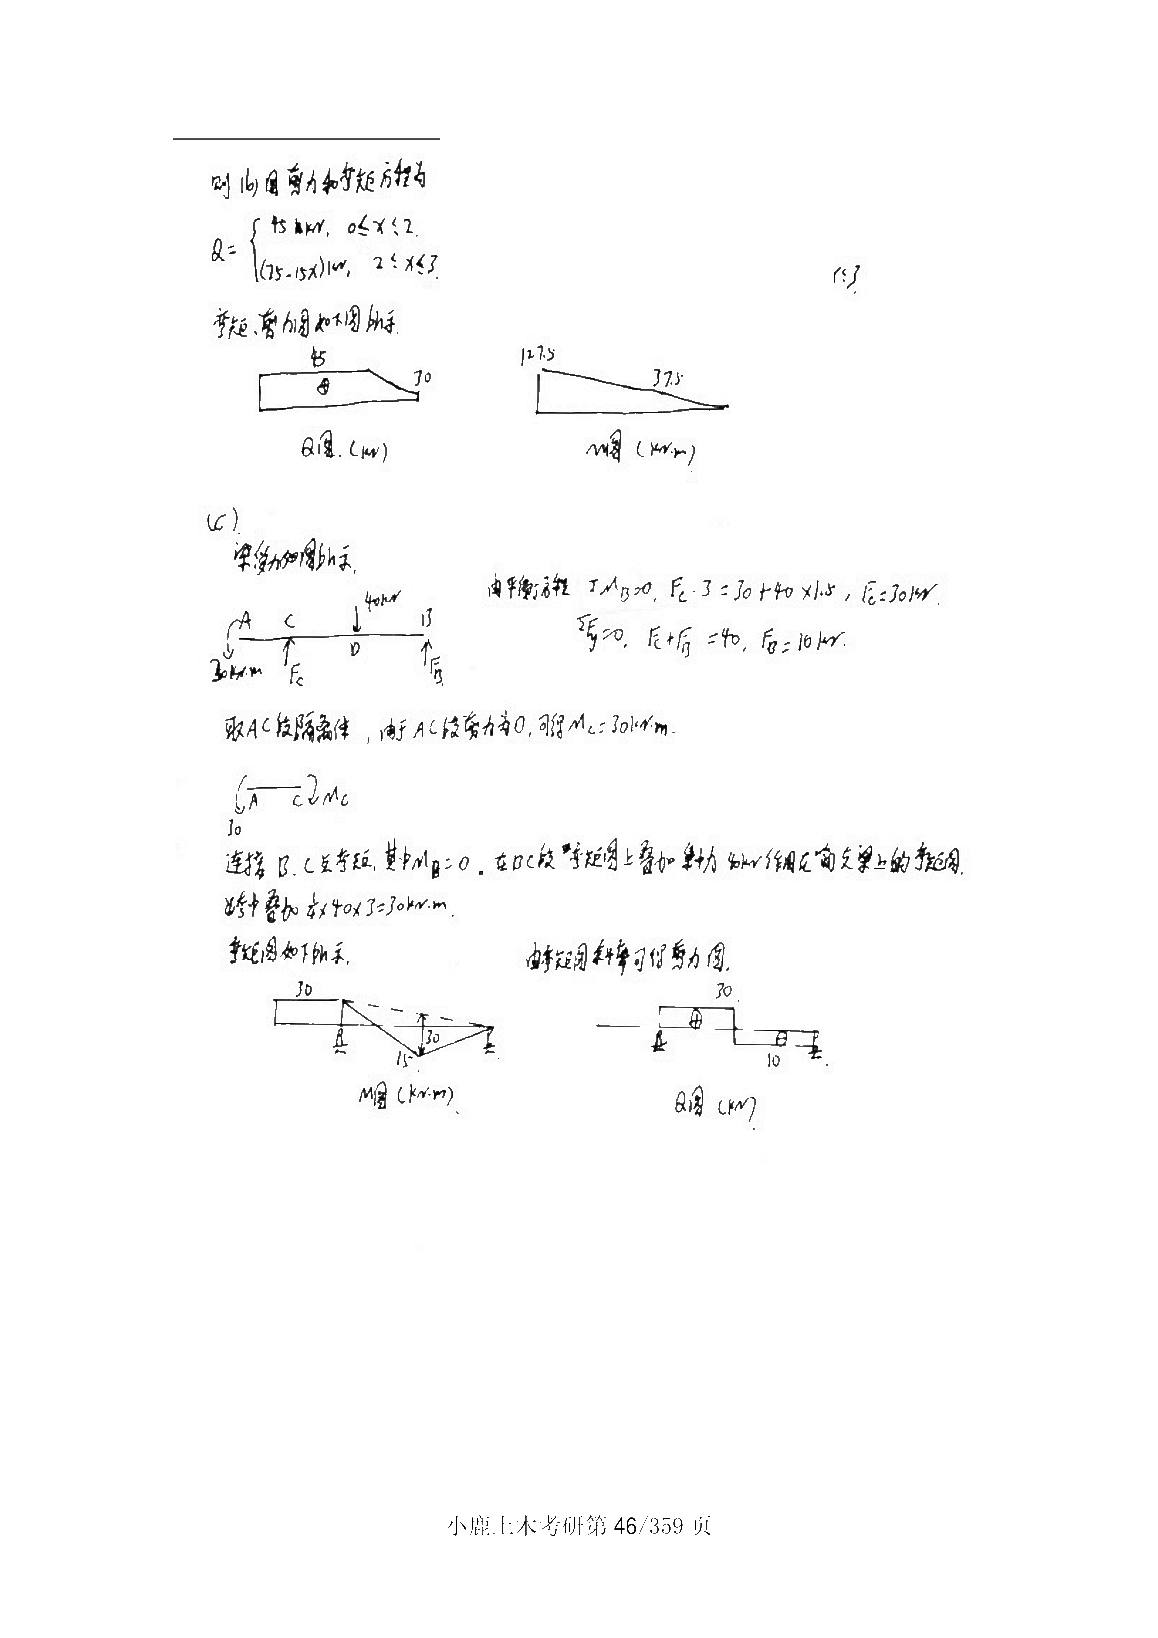
\includegraphics[width=0.92\textwidth]{figures/src06_p004.jpg}
\caption{结构力学基础与技巧班第3次作业（材料力学回顾） 第 4 页清理图形页}
\end{figure}
\subsection*{第 5 页转写}
取整体陷多压,由MA=0,0.2*bx5 +9一后$\times$10=0,罚后：1.4km.

Tg=0, +后=azxo, Fa= 0.byw.

点处作因有集功偶，改四目内定受,

取 Ct例到吐终随务体

由Mc=0, Mc$\pm$+后x2 -0.2x2|20, Mb: -24 km(

1.6

Mackm)

由于净上无转力个,改两力国乱突度,打条直理,邻节为a2,

.6
\begin{figure}[H]\centering
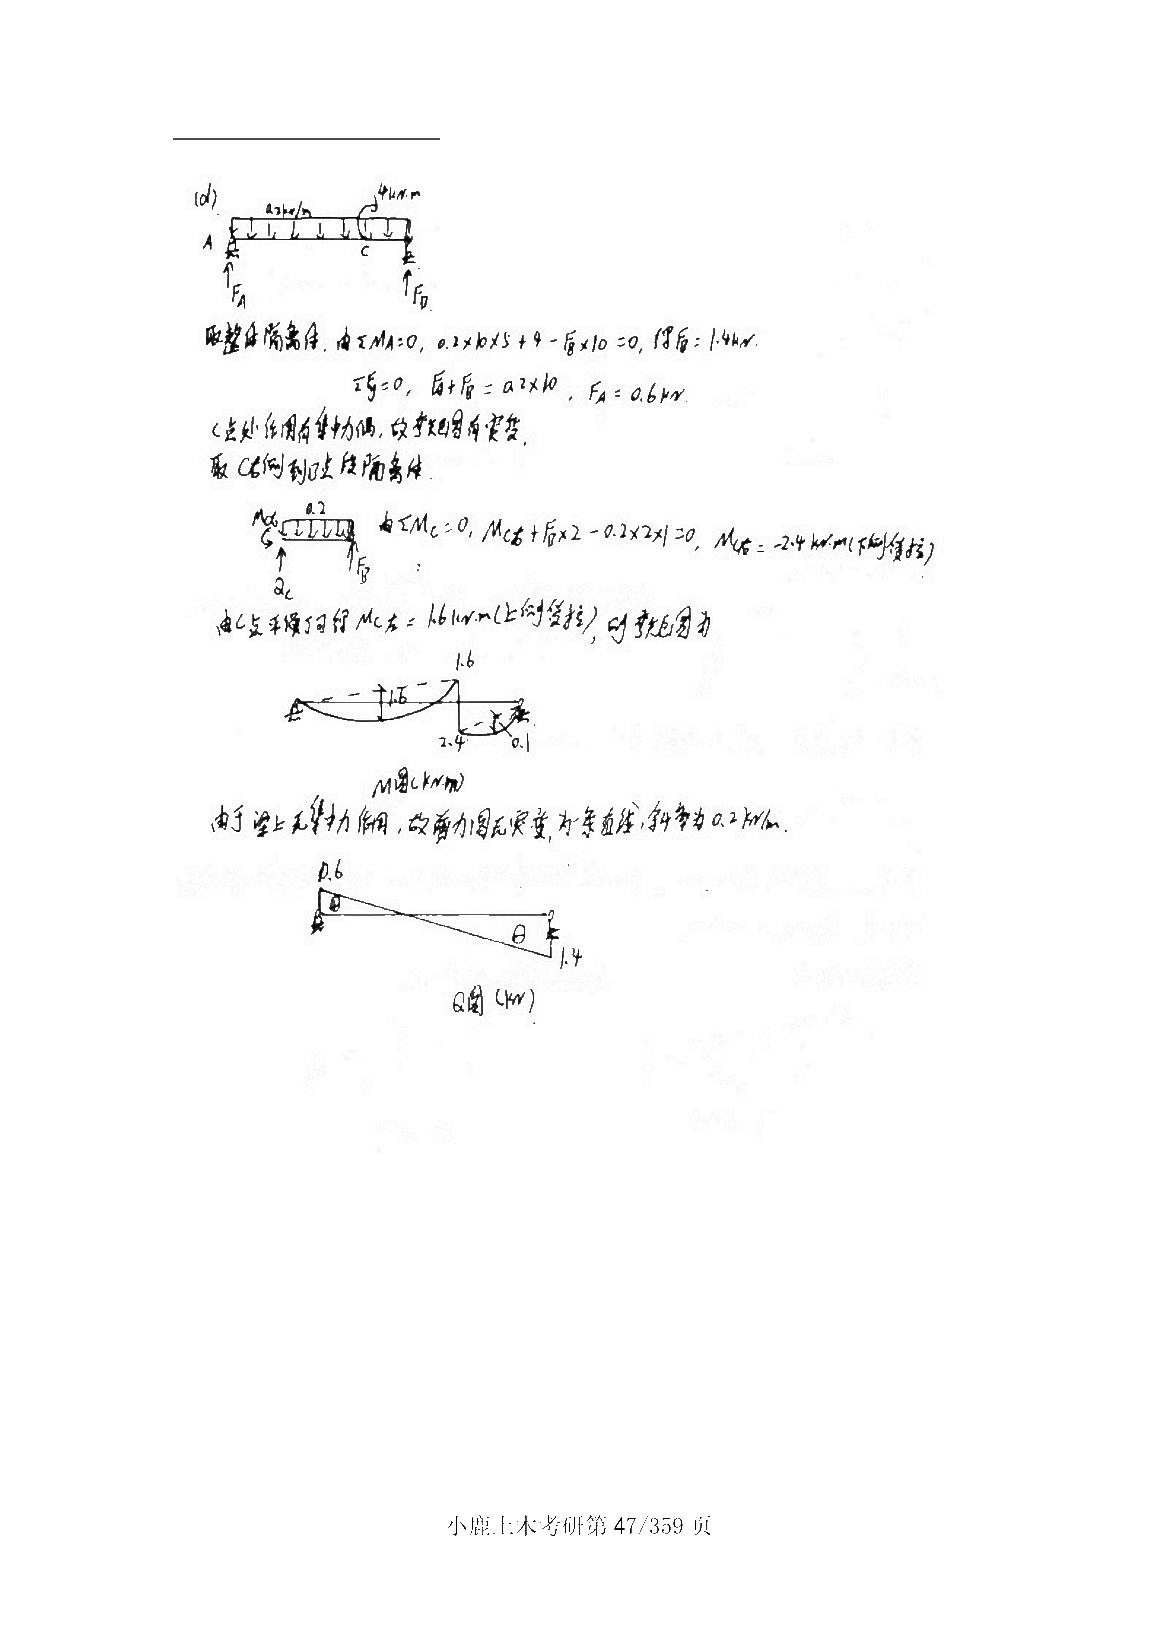
\includegraphics[width=0.92\textwidth]{figures/src06_p005.jpg}
\caption{结构力学基础与技巧班第3次作业（材料力学回顾） 第 5 页清理图形页}
\end{figure}
\subsection*{第 6 页转写}
(e)

Zoky

20ko.m

现整结为随禽体, 对A取知,由g0, b+20+20$\times$2 -后了0, 后=2 M,

50, 丙+20-斤=0 ,反=2.

死AC转隔备伴

mc 0, Mc +2 2 - 620, Mc=2 kmm,

00,Q左+220,Qu=2.

别本接 CA女梦延和C女考短即M由m图钟节月理Q限

体随病体,由Ms0, E-4$\alpha$ - . a. a 0, 后:

由C依隔务件，

Me-o, Me = L9a*.

连择 A.c点步, M,由 m明针抑可得 Qr.
\begin{figure}[H]\centering
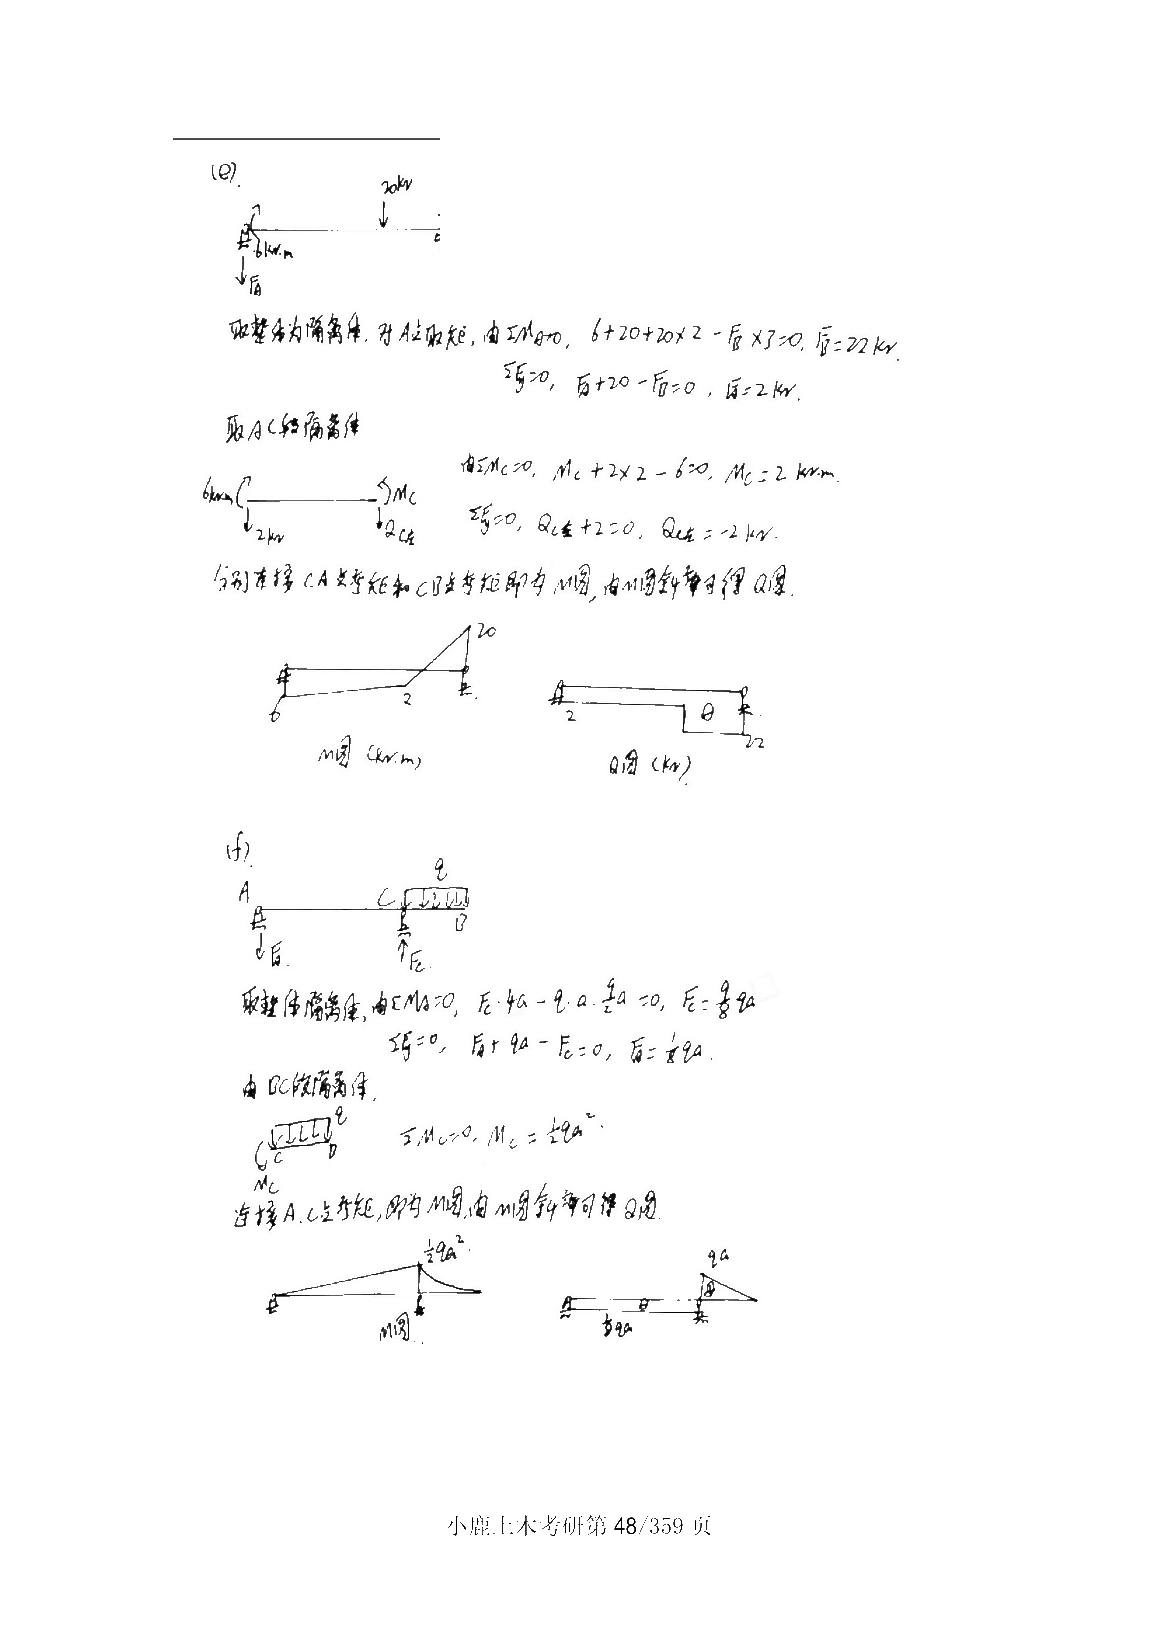
\includegraphics[width=0.92\textwidth]{figures/src06_p006.jpg}
\caption{结构力学基础与技巧班第3次作业（材料力学回顾） 第 6 页清理图形页}
\end{figure}
\subsection*{第 7 页转写}
(0)

体体为随多4,等取短,由Ms10, MA =5$\times$1$\times$ 2 =10km

由Ac剪力为,日约 AL统为5W,则M=2.5Wl上图台均)

M图 ( ks.m)

Ac 经显剪力不复,为上kv, UC收力争为的师构获k小 51m/n

binm

线巨为$^\circ$,刚为0,0.

最整体隔离库,20.Ms=15X1+02m.m

连 A.C禁即为M间,禁单可K口剪力目.

m)( kmm)
\begin{figure}[H]\centering
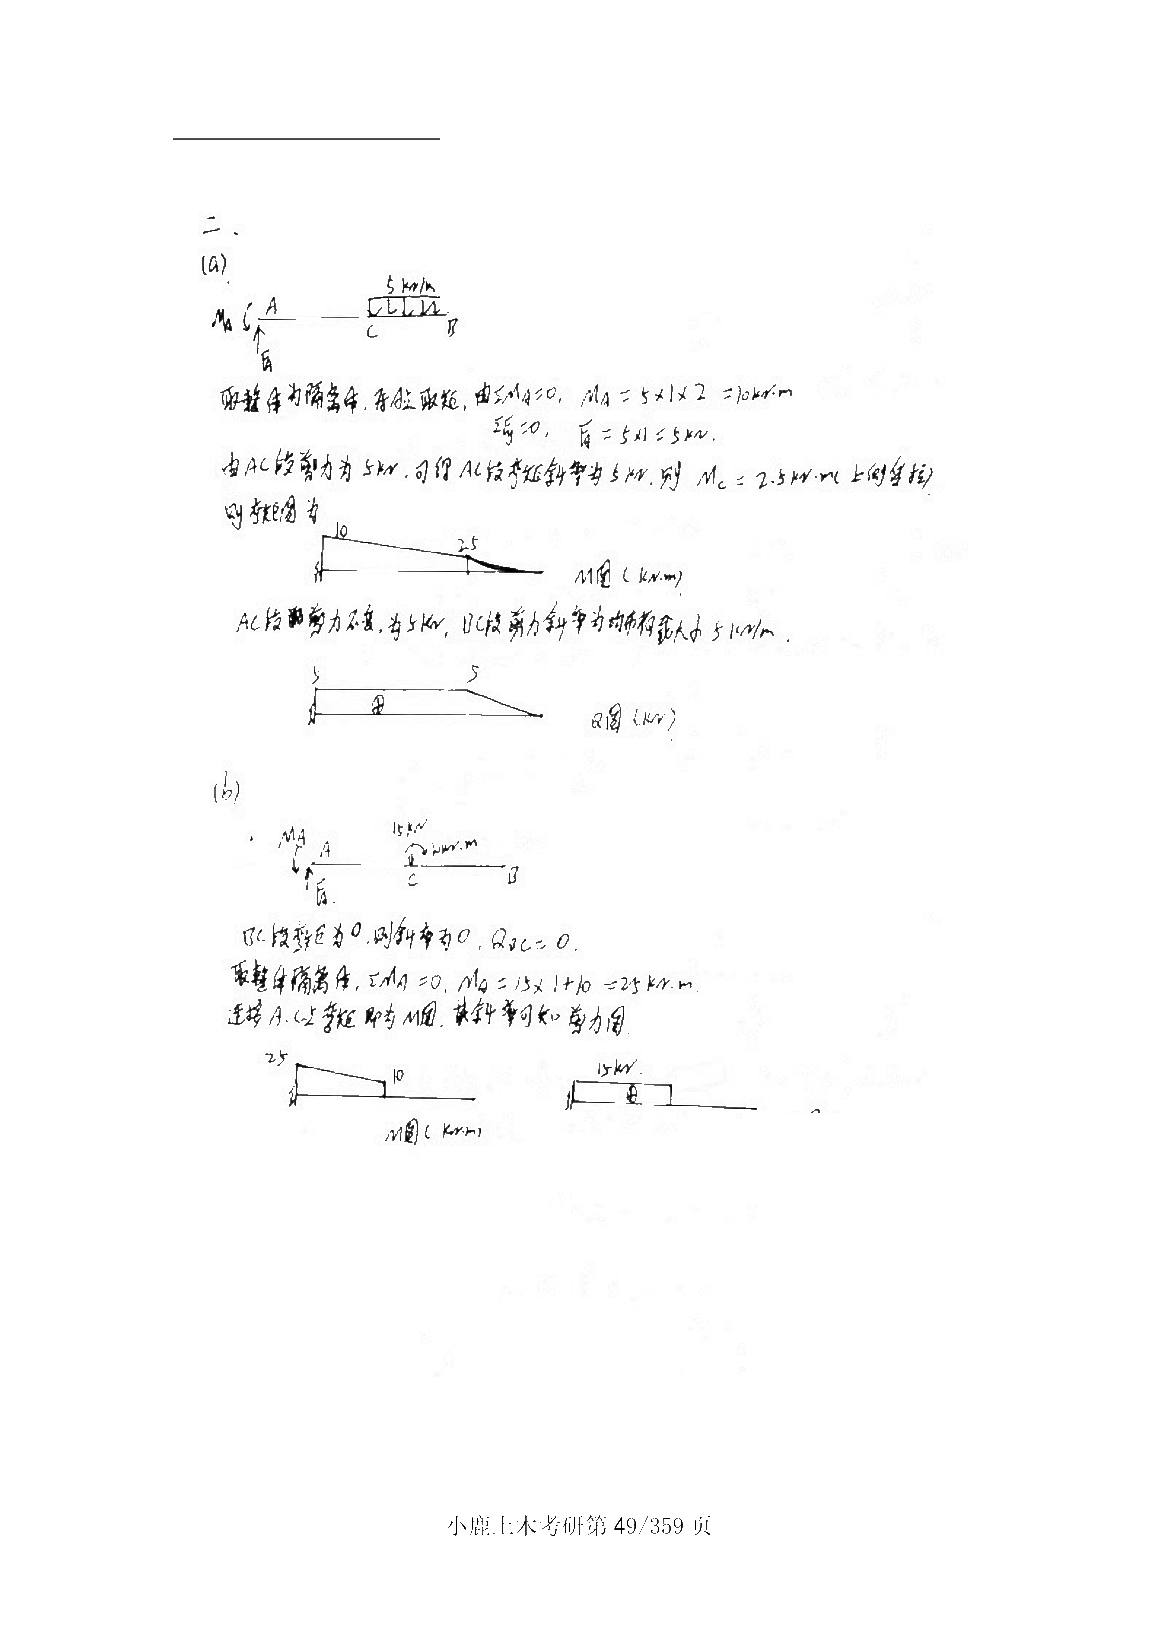
\includegraphics[width=0.92\textwidth]{figures/src06_p007.jpg}
\caption{结构力学基础与技巧班第3次作业（材料力学回顾） 第 7 页清理图形页}
\end{figure}
\subsection*{第 8 页转写}
尾QALa，Ms>0,行 MeA* (扫)=Mo)

连好 C.D梦柜,一加。 均布药较作用在简支甲上的效目的为 ml,

Qp，C剪力+为,

99

(p)

整体临生, 1Me= 0, 2Ne-Mo \textasciitilde{}后双$\ge$0 , 后=笼,

由 AC转力为\&h签，2g,月M cA= 上与维控)

2Me.
\begin{figure}[H]\centering
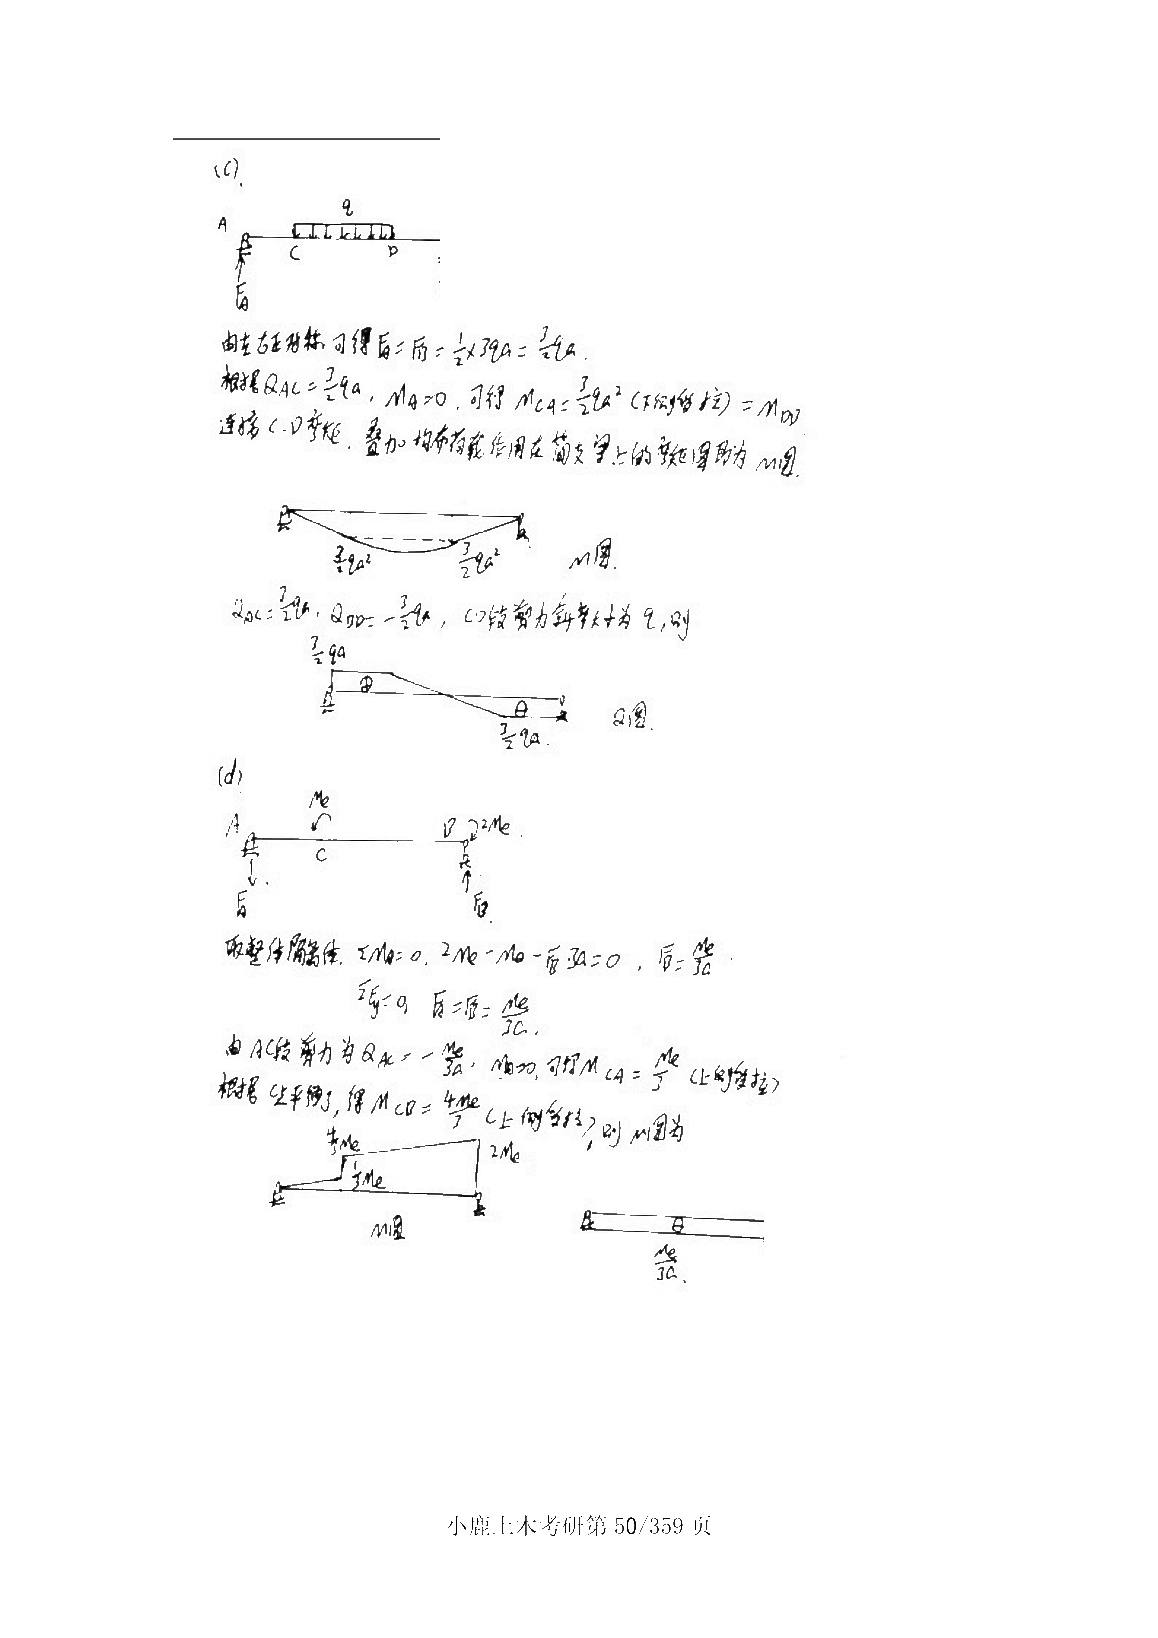
\includegraphics[width=0.92\textwidth]{figures/src06_p008.jpg}
\caption{结构力学基础与技巧班第3次作业（材料力学回顾） 第 8 页清理图形页}
\end{figure}
\subsection*{第 9 页转写}
必整体陷离体，由工Ma0,4+4$\times$4X2+20后420,后=)41W

500，后=4，后2

目直培得到样(因, b如/h示

左达符符,可得后=后二完.

相据QAL=F，Maz0,传MeR=fa (下例命

0, Q=F

根据净co较力日得Moc=多Fa (上例实),
\begin{figure}[H]\centering
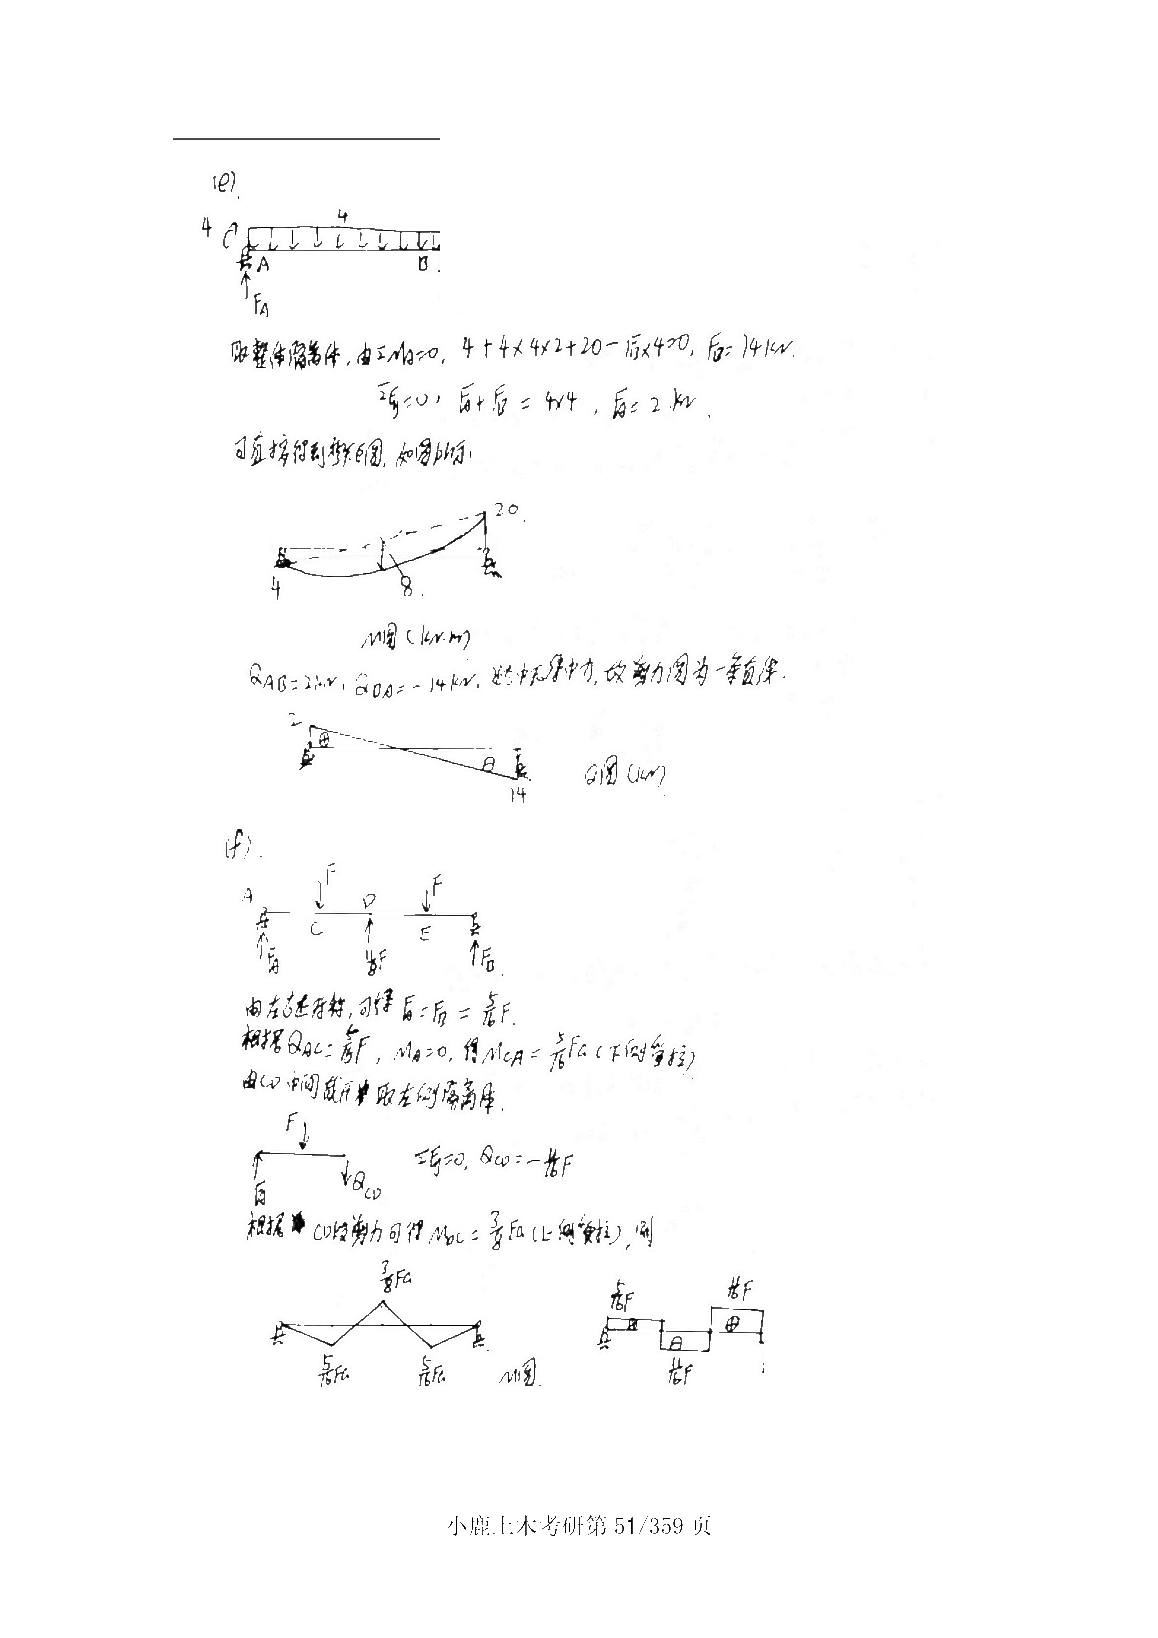
\includegraphics[width=0.92\textwidth]{figures/src06_p009.jpg}
\caption{结构力学基础与技巧班第3次作业（材料力学回顾） 第 9 页清理图形页}
\end{figure}
\subsection*{第 10 页转写}
整体离体,由M00, 后$\times$2=2$\times$1x$\pm$,后k

0, Fz ],

M (km.m)

BC粒力为Qpc-至, BA=是kn, Ac结力国钟牌力2IWh,可力同为

(n)

取 C左网动A点段隔离体

IMe=0, Mes +2 -1oX2x) 20, MeA:-54o /mm

0,Q$\pm$+10x2一月0,Qc:26oyv.

Igo, +od sbw.
\begin{figure}[H]\centering
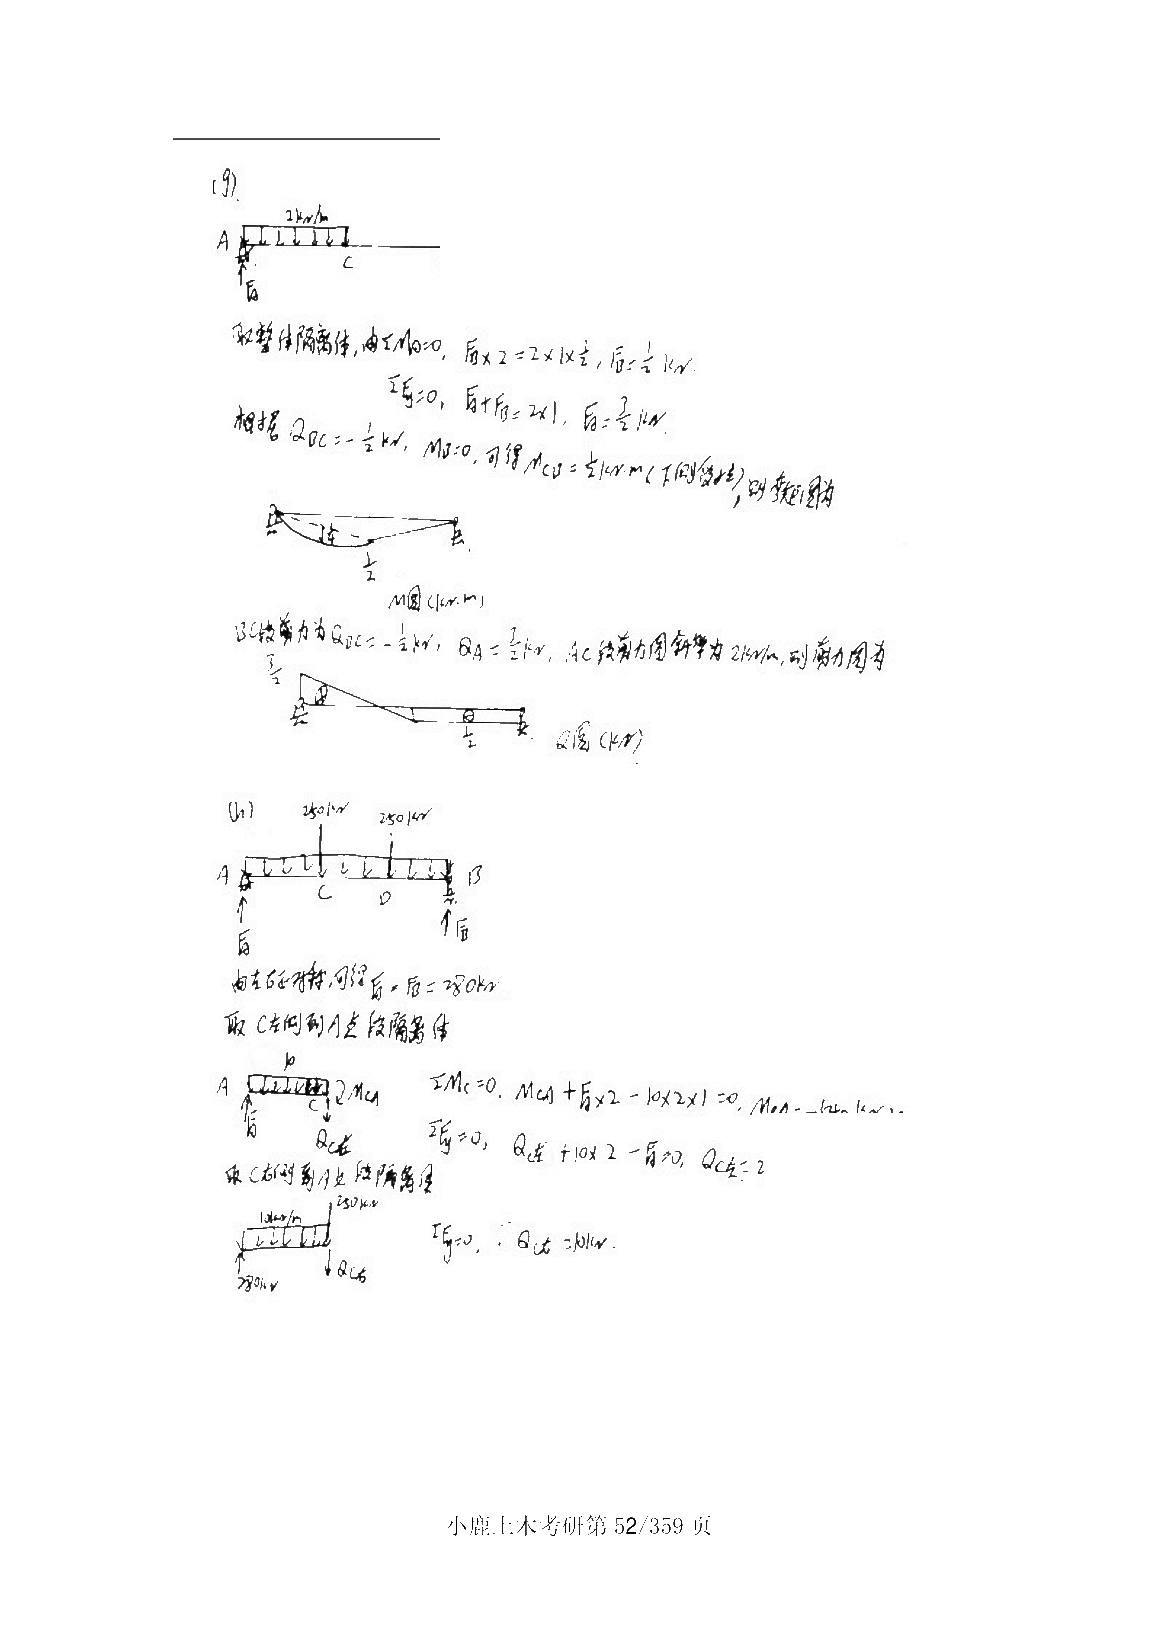
\includegraphics[width=0.92\textwidth]{figures/src06_p010.jpg}
\caption{结构力学基础与技巧班第3次作业（材料力学回顾） 第 10 页清理图形页}
\end{figure}
\subsection*{第 11 页转写}
m国 ( kn)

给构好格下，力月为符，

(0)

双级确体，升点取炬，可得

Mg:0,Qca+9a.4=0,Qc=-90

Mg=96.4=96

199

取Ac海体

由Mg=0,M=9a.g-，9*例)

881

M'BAC

0,Qac=9A+\&c=0
\begin{figure}[H]\centering
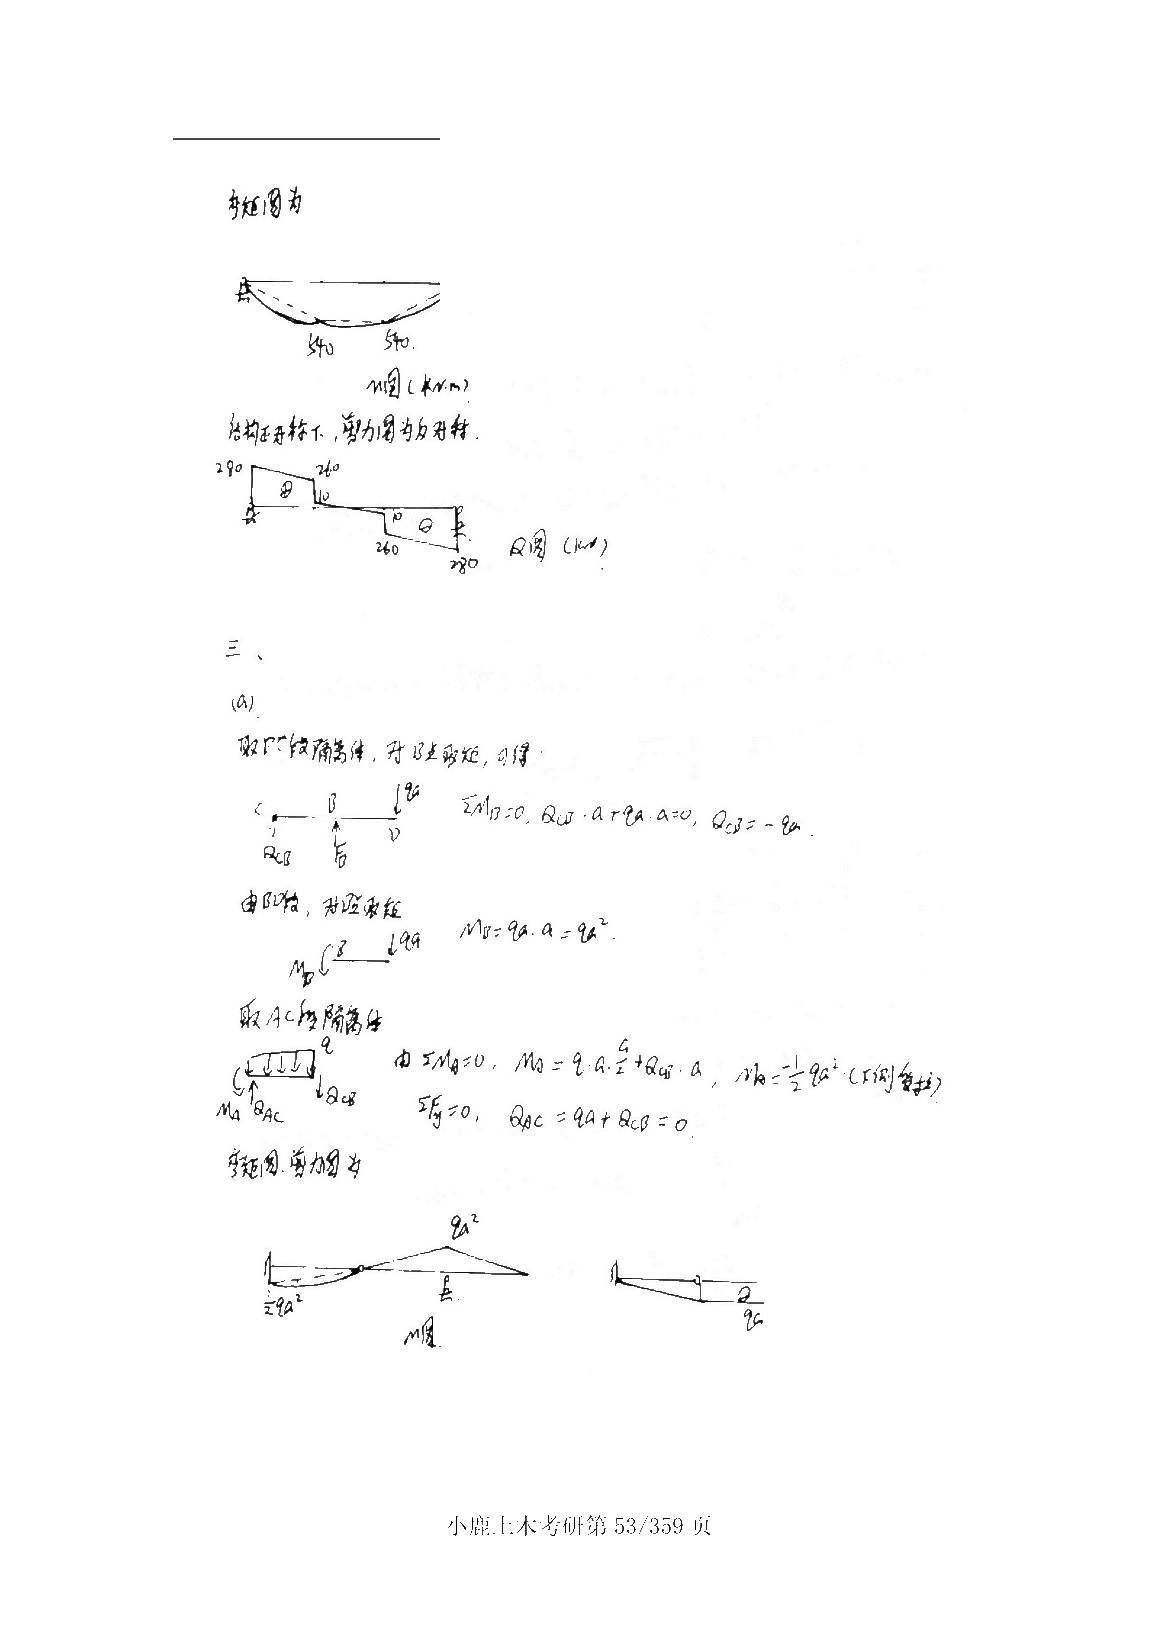
\includegraphics[width=0.92\textwidth]{figures/src06_p011.jpg}
\caption{结构力学基础与技巧班第3次作业（材料力学回顾） 第 11 页清理图形页}
\end{figure}
\subsection*{第 12 页转写}
(b),

取AC 段防离体

由e20,后=08c,放A力，

取险左例有C隔件

由Mzo, M -a.= ga',

5=0,Q3c=-9么.

9A.
\begin{figure}[H]\centering
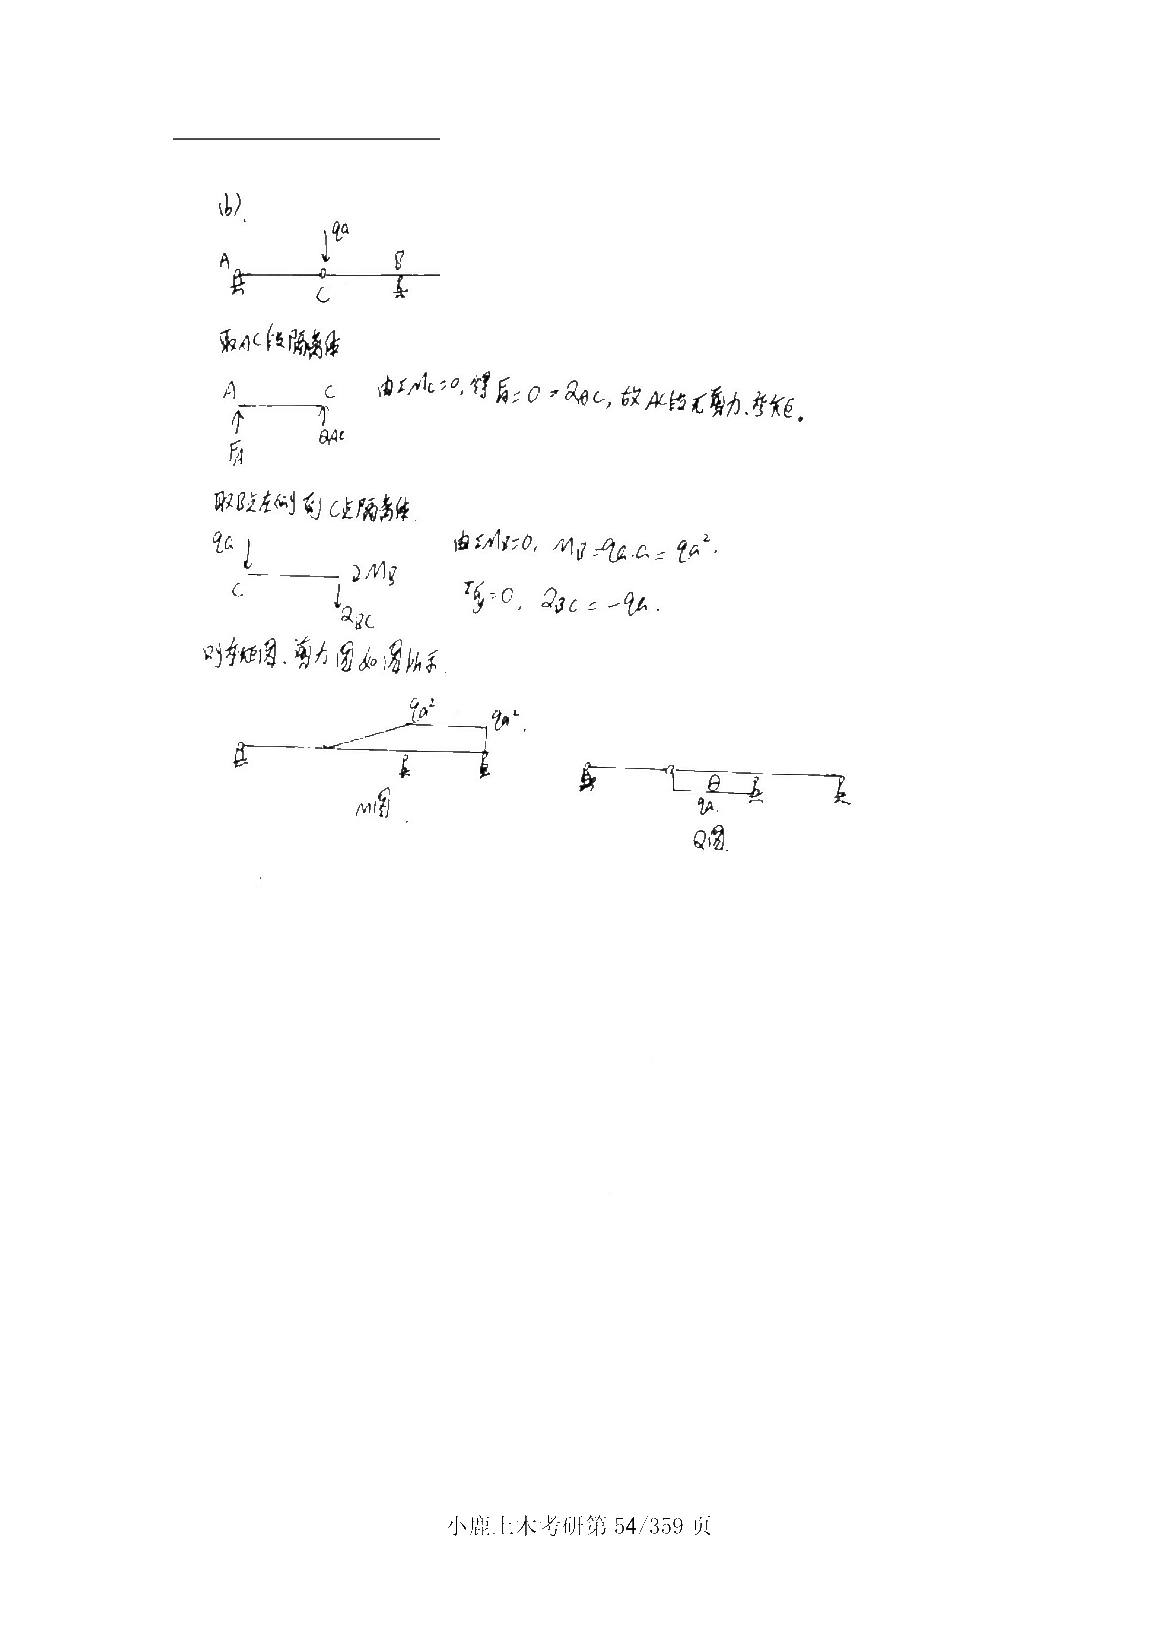
\includegraphics[width=0.92\textwidth]{figures/src06_p012.jpg}
\caption{结构力学基础与技巧班第3次作业（材料力学回顾） 第 12 页清理图形页}
\end{figure}
